% !TEX encoding = UTF-8 Unicode
% !TEX program = pdflatex
% !TEX spellcheck = en_US


% In order to correctly compile this document,
% execute the following commands:
% 1. pdflatex
% 2. pdflatex
% 3. pdflatex



\documentclass[amsthm,ebook]{saparticle}

% IF YOU USE PDFLATEX
\usepackage[utf8x]{inputenc}
% if you write in english and in greek
\usepackage{ucs}
\usepackage[greek,english]{babel}
\languageattribute{greek}{polutoniko}

% IF YOU USE XELATEX
%\usepackage{polyglossia}
% if you write in italian
%\setmainlanguage{italian}
% If you want put some ancient greek:
%\setotherlanguage[variant=polytonic]{greek}
%\newfontfamily{\greekfont}[Ligatures=TeX]{Palatino Linotype}

% dummy text (remove in a normal thesis)
% remove if not necessary
\usepackage{siunitx}
%Natbib for bibliography management
\usepackage[authoryear]{natbib}
% custom commands
\newcommand{\bs}{\textbackslash}

%%%%%%%%
%TITLE:%
%%%%%%%%

\title{Digital enhancement of the ``Paolo Orsi'' museum: a Google Street View 360° pilot project tour}
\author[catania]{Elisa Bonacini\corref{first}}
\cortext[first]{Corresponding author. Email: e_bonacini@hotmail.com; elisa.bonacini@unict.it}
\address[catania]{Humanities Department, University of Catania; IEMEST (Istituto Euro Mediterraneo di Scienze e Tecnologie), Palermo, Italy}
\date{2015-12-11}
\begin{document}
 
\maketitle
\begin{abstract}
The aim of this paper is to present the pilot project in progress at the ``Paolo Orsi'' Archaeological Museum
(Syracuse, Italy). Thanks to a free partnership with Google Business Photos, we have managed to map the entire museum
for a online 360° tour on Google Street View. A dozen archaeological finds have been selected for 360° virtual tours,
provided with descriptive sheets. Among them the beautiful `inscription of Nassiane', from the Catacombs of San
Giovanni in Syracuse, has been selected.
\end{abstract}
\keywords{Google, Sicily, Sicilian Cultural Heritage, Virtual Museum, Virtual tour, Digital Heritage} 


\section{The ``Paolo Orsi'' Archaeological Museum}


The ``Paolo Orsi'' Regional Archaeological Museum of Syracuse, together with the ``Antonino Salinas'' Regional
Archaeological Museum in Palermo, is the most important Sicilian archaeological museum and it is one of the most
important and richest archaeological museums in Italy. 

The National Archaeological Museum of Syracuse was born by a royal decree in 1878, known as ``national'' for its
collections’ importance and size. Well-placed inside the historical palace in the Cathedral Square on Ortigia island,
it was directed by Paolo Orsi from 1895 to 1934. 

The archaeological collection has been enlarged by over 70 years of archaeological research making it necessary to move
the collection to a new museum space. Designed by the architect Franco Minissi, the new museum was built in the Villa
Landolina garden between 1967 and 1986 and inaugurated in January 1988. The collection consists of artefacts from the
prehistoric, Greek, Roman and Christian periods found in archaeological excavations in Syracuse and in other Sicilian
sites. The museum space is divided in three levels (floor 1, 2 and basement), distributed around a central space which
is dedicated to the history of the museum and temporary exhibitions. First level is divided in three sectors (A – C)
and testifies the history of central-eastern Sicily from prehistoric ages to the Greek one. On the upper floor, sectors
D and F were inaugurated in 2006 and contain finds from the Hellenistic-Roman and Christian periods. Section E will
open next year with findings from sites in central-eastern Sicily (as Centuripe, Morgantina, Tindari and so on).
Moreover, a precious and unique collection of coins and medals from archaic to the medieval age is located in the
basement, opened in 2010.




\section{The project: reasons and birth}


This project born from the desire to fill the deep gap in the promotion and enhancement of Sicilian cultural heritage. 

Sicily has the highest number of UNESCO heritage sites (7/51 in total\footnote{1997: Valley of Temples in Agrigento;
1997: Villa del Casale; 2000: Eolian Islands; 2002: Late Baroque Towns of the Val di Noto (South-Eastern Sicily); 2005:
Syracuse and the rock necropolisof Pantalica; 2013: Mount Etna; 2015: Arab-Norman sites, Palermo and the Cathedral
Churches of Cefalù and Monreale.}) and of UNESCO intangible cultural heritage (3/6\footnote{2008: Opera dei Pupi,
Sicilian puppet theatre; 2013: Mediterranean diet (transnational); 2014: Traditional agricultural practice of
cultivating the `vite ad alberello' (head-trained bush vines) of the community of Pantelleria.}) in Italy and in the
world. Infact, Sicily has some of the largest and most important archaeological sites in the world: the temple of
Concordia in Agrigento, for its exceptional state of preservation has become the symbol of UNESCO itself.

Despite of this, Sicilian cultural heritage struggles to be present on Google’s platforms such as Google Art Project and
others, as it should, compared to other Italian cultural sites \citep{Bonacini2013} \citep{Bonacini2014}).

It is not so difficult to explain where the difference between the island and its mother country comes from. Sicily has
the status of independent region, therefore it has an exclusive competence in the field of regional cultural heritage.
Sicilian heritage is released from any convention that the Italian Ministry of Cultural Heritage and Tourism has signed
since 2009 with Google. The Regional Department of Culture and Sicilian Identity has never bothered to solve this
really huge gap regarding its cultural heritage and landscapes.

In Street View Gallery\footnote{\url{https://www.google.com/maps/views/streetview?gl=us}.}, which now has contributed a great
number of users from all over the world, thousands are the spherical and geo located photos of Italian places. However,
tightening the selection to ``Landmarks of Italy''
\footnote{\url{https://www.google.com/maps/views/streetview/italy-highlights?gl=us}.}, Sicily has only 9 spherical photos,
showing the beaches of the Aeolian Islands (7), the islands of Favignana (1) and Marettimo (1). 

Among Art Project’s 605 museum collections\footnote{\url{https://www.google.com/maps/views/streetview/art-project?gl=it}.}, 47
are Italian, especially relevant to Rome, Turin, Venice and Milan. One of these, not the best artistic production, is a
Sicilian contemporary collection, relevant to the International Festival of Street Artists in Giardini Naxos (Me). No
other Sicilian museum, collection or archaeological site has been included in Art Project.

Browsing on the Street View Gallery, 21 sites are all over inscribed on the World Wonders
Project\footnote{\url{https://www.google.com/maps/views/streetview/world-wonders-project?gl=it}.}: for Italy, only Pompeii
and the historic center of Florence are inscribed in this still restricted list. Many more sites can be visited
virtually from the same project linked on Google Cultural Institute’s
website\footnote{\url{www.google.com/intl/it/culturalinstitute/worldwonders/}. }: 172 sites in the world, 22 in Italy and,
finally, 2 of them in Sicily. Until last year the Unesco site of the baroque town Val di Noto was the only one in
Sicily; currently Mount Etna, has been added. 

Google organized its Google Camp 2014 and 2015 editions by selecting as exceptional locations two of the most evocative
archaeological sites in the world, Selinunte and Agrigento. Nevertheless the beauty and heritage of Sicily, ironically,
is not on Google’s platforms.

This project was born in collaboration with Mr. Gianfranco Guccione, a certified Google Business Photo photographer,
while he was working as a freelance consultant at the General Direction of the Regional Department for Cultural
Heritage and Sicilian Identity in 2014. He proposed to realize the Street View mapping of a museum and an
archaeological site in Sicily, considering the possibility of creating ``augmented'' virtual tours (3D virtual tours of
objects displayed in museum’s windows and virtual aerial tours, with the addition of text and audio descriptions). 

The profound reason of this project consists in an effort to bridge this gap, ``increasing'' fruition and enhancement of
Sicilian cultural heritage. 

With the agreement between the General Direction of the Regional Department for Cultural Heritage and Sicilian Identity
and the European Coordination of Google Business Photo, it was decided to choose as a sample of this project two
cultural regional institutions, the ``Paolo Orsi'' Museum in Syracuse and the Valley of the Temples in Agrigento, both
UNESCO sites since 2005 and 1997. The project was then structured as a research fellow project at the University of
Catania and carried out by the present writer in close collaboration with Mr. Guccione. 

The first part of the project at the ``Paolo Orsi'' Museum, which we will discuss here, is about to be completed. The
second part at Valley of the Temples in Agrigento is going to start.




\subsection{The 360° tour on Google Maps: some technical data}


A large photographic survey began in August 2014, with the aim of mapping all areas of the first and second level open
to visitors (only the collection of coins and medals, for security reason, has not yet been photographed). 

A total of 3.924 shots to get about 327 360° virtual tours have been made using a mobile station made up by a reflex
camera with fisheye type camera lens, tripods with panoramic head. Because of the peculiarity of the light in the
different museum’s sectors, it was necessary to adjust the brightness each time. The windows in the winding path often
reflect one another and precautions were taken to avoid, as far as possible, those refractions.

Once loaded on Google’s software Business Photos, the pack of images from the 327 virtual tours were geo located in
Google Maps Street View, mounted avoiding defects of sight between the images. 

The 360° virtual tour makes it possible browsing the entire museum and its collection, between levels connected by
arrows, placed online at the link \url{https://goo.gl/maps/oagnd8urP1H2} (for the first level) and
\url{https://goo.gl/maps/vrpDfuPPgwM2} (for the second level). As you can see in Fig.~\ref{fig:1}, by clicking on the first link,
the remote user can enter the museum through the Street view panel: the 360° virtual tour begins at the entrance and
the user can browse moving with the directional arrows, between sectors and levels.

The project provided the opportunity to carry out 360° virtual tours of some exposed archaeological finds, like an
``augmented'' virtual tour, certainly innovative compared to what Google’s platforms provide. 

Art Project, for example, allows you to view points of interest along the path in a museum, but captions are short and
photos are static. A pilot initiative has been recently launched featuring the possibility to in-browse almost 300 3D
photos of objects from the collections of six cultural institutions in the world. However 242 of these consist of scans
of animal skulls (pieces of nature, not works of art) from the California Academy of Science collection; 22 objects of
art come from Museo d’Arte Orientale (the only Italian cultural institution to join the project until now). These 3D
objects, described by short captions, are available to users to be rotated and zoomed. The aim of this new Google’s
project is to begin building the most important and largest database of 3D scan art of works worldwide. 

\begin{figure}[!bp]
\centering
 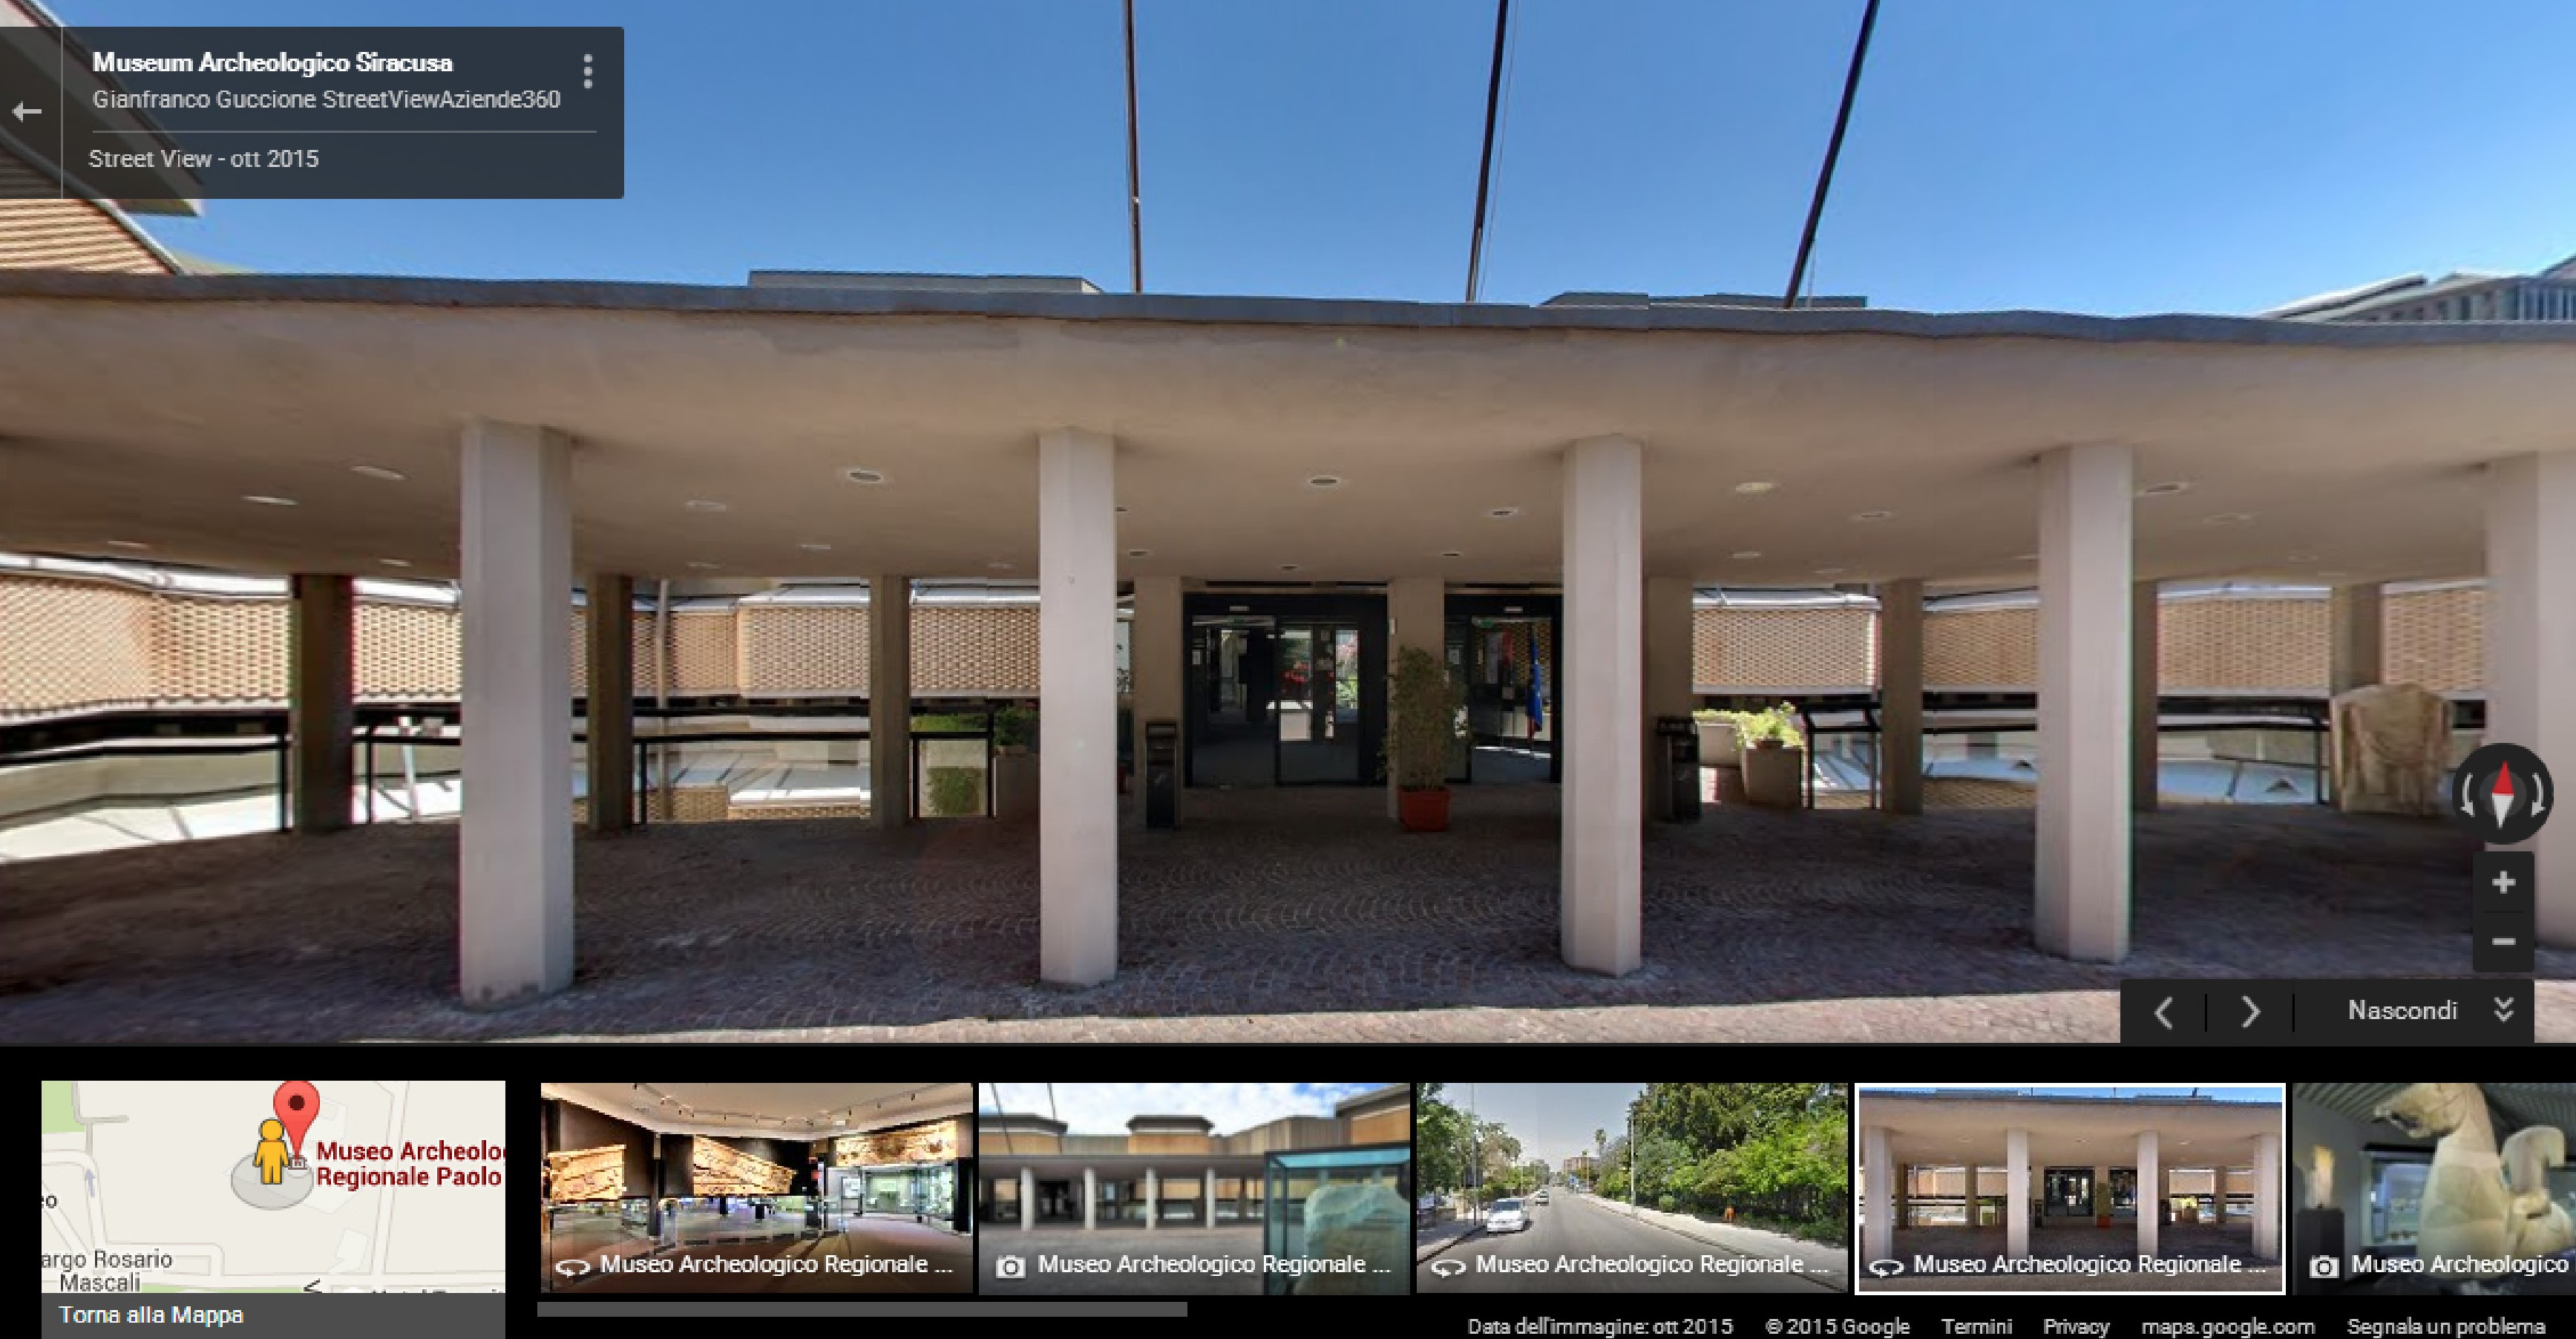
\includegraphics[width=\columnwidth]{EAGLE2016BONACINIPilotprojectatPaoloOrsiMuseum-img001.jpg}
\caption{The virtual entrance to Archaeological Museum ``Paolo Orsi'' on Google Street View. }
\label{fig:1}
\end{figure}


As for the displaying on Google Maps of the 360° virtual tour of the objects, we must specify that Maps so far does not
support the integration of menus, captions, photos, video, info inside the Street View virtual tour technology.
Infact,it is only allowed navigation in 360°, ie a virtual walk.

We tried to find an answer in order to show on Maps all the information, captions, maps, levels and 360° virtual tour of
objects. Thanks to customized i-frame we made these virtual tours possible with their captions and the maps with
different levels and clickable points of interest, adding them to the existing virtual tour of the Museum, already on
Maps, through a link containing the Google mapping of the Museum. In this way the virtual tour of the Museum - made
with Google standards - is ``augmented'' by another virtual walk much more exhaustive, located via link on the Google
Maps board of the Museum, where you can view all these additional items.

Both the virtual tour of the museum and the virtual tour of the objects will also be placed on the Museum's website, on
the Regional Department for Cultural Heritage and Sicilian Identity portal
(\url{http://www.regione.sicilia.it/beniculturali/museopaoloorsi/}). Because of the profound principle that this non-profit
project would improve the visibility and promotion of Sicilia Cultural Heritage, the Museum’s virtual tour and its
reproductions belong to Google; Museum’s objects virtual tours, instead, belong to Paolo Orsi Museum, which is free to
reuse them. 




\subsection{The ``Paolo Orsi'' Museum 360° tour}


Coming from Sector A, after turning around a couple of casts of dwarf elephants from Spinagallo cave (Syracuse), a
remote user can see the displayed artifacts, starting with Neolithic phase of Stentinello (VI millennium B.C.) to reach
the great exhibition space dedicated to Bronze age: Ancient Bronze age (facies of Castelluccio), Middle Bronze age
(facies of Thapsos), Late Bronze age (facies of Pantalica) and Final Bronze age (facies of Finocchito), where \ the
large containers from Thapsos and Pantalica necropolis.

\begin{figure}[!bp]
\centering
 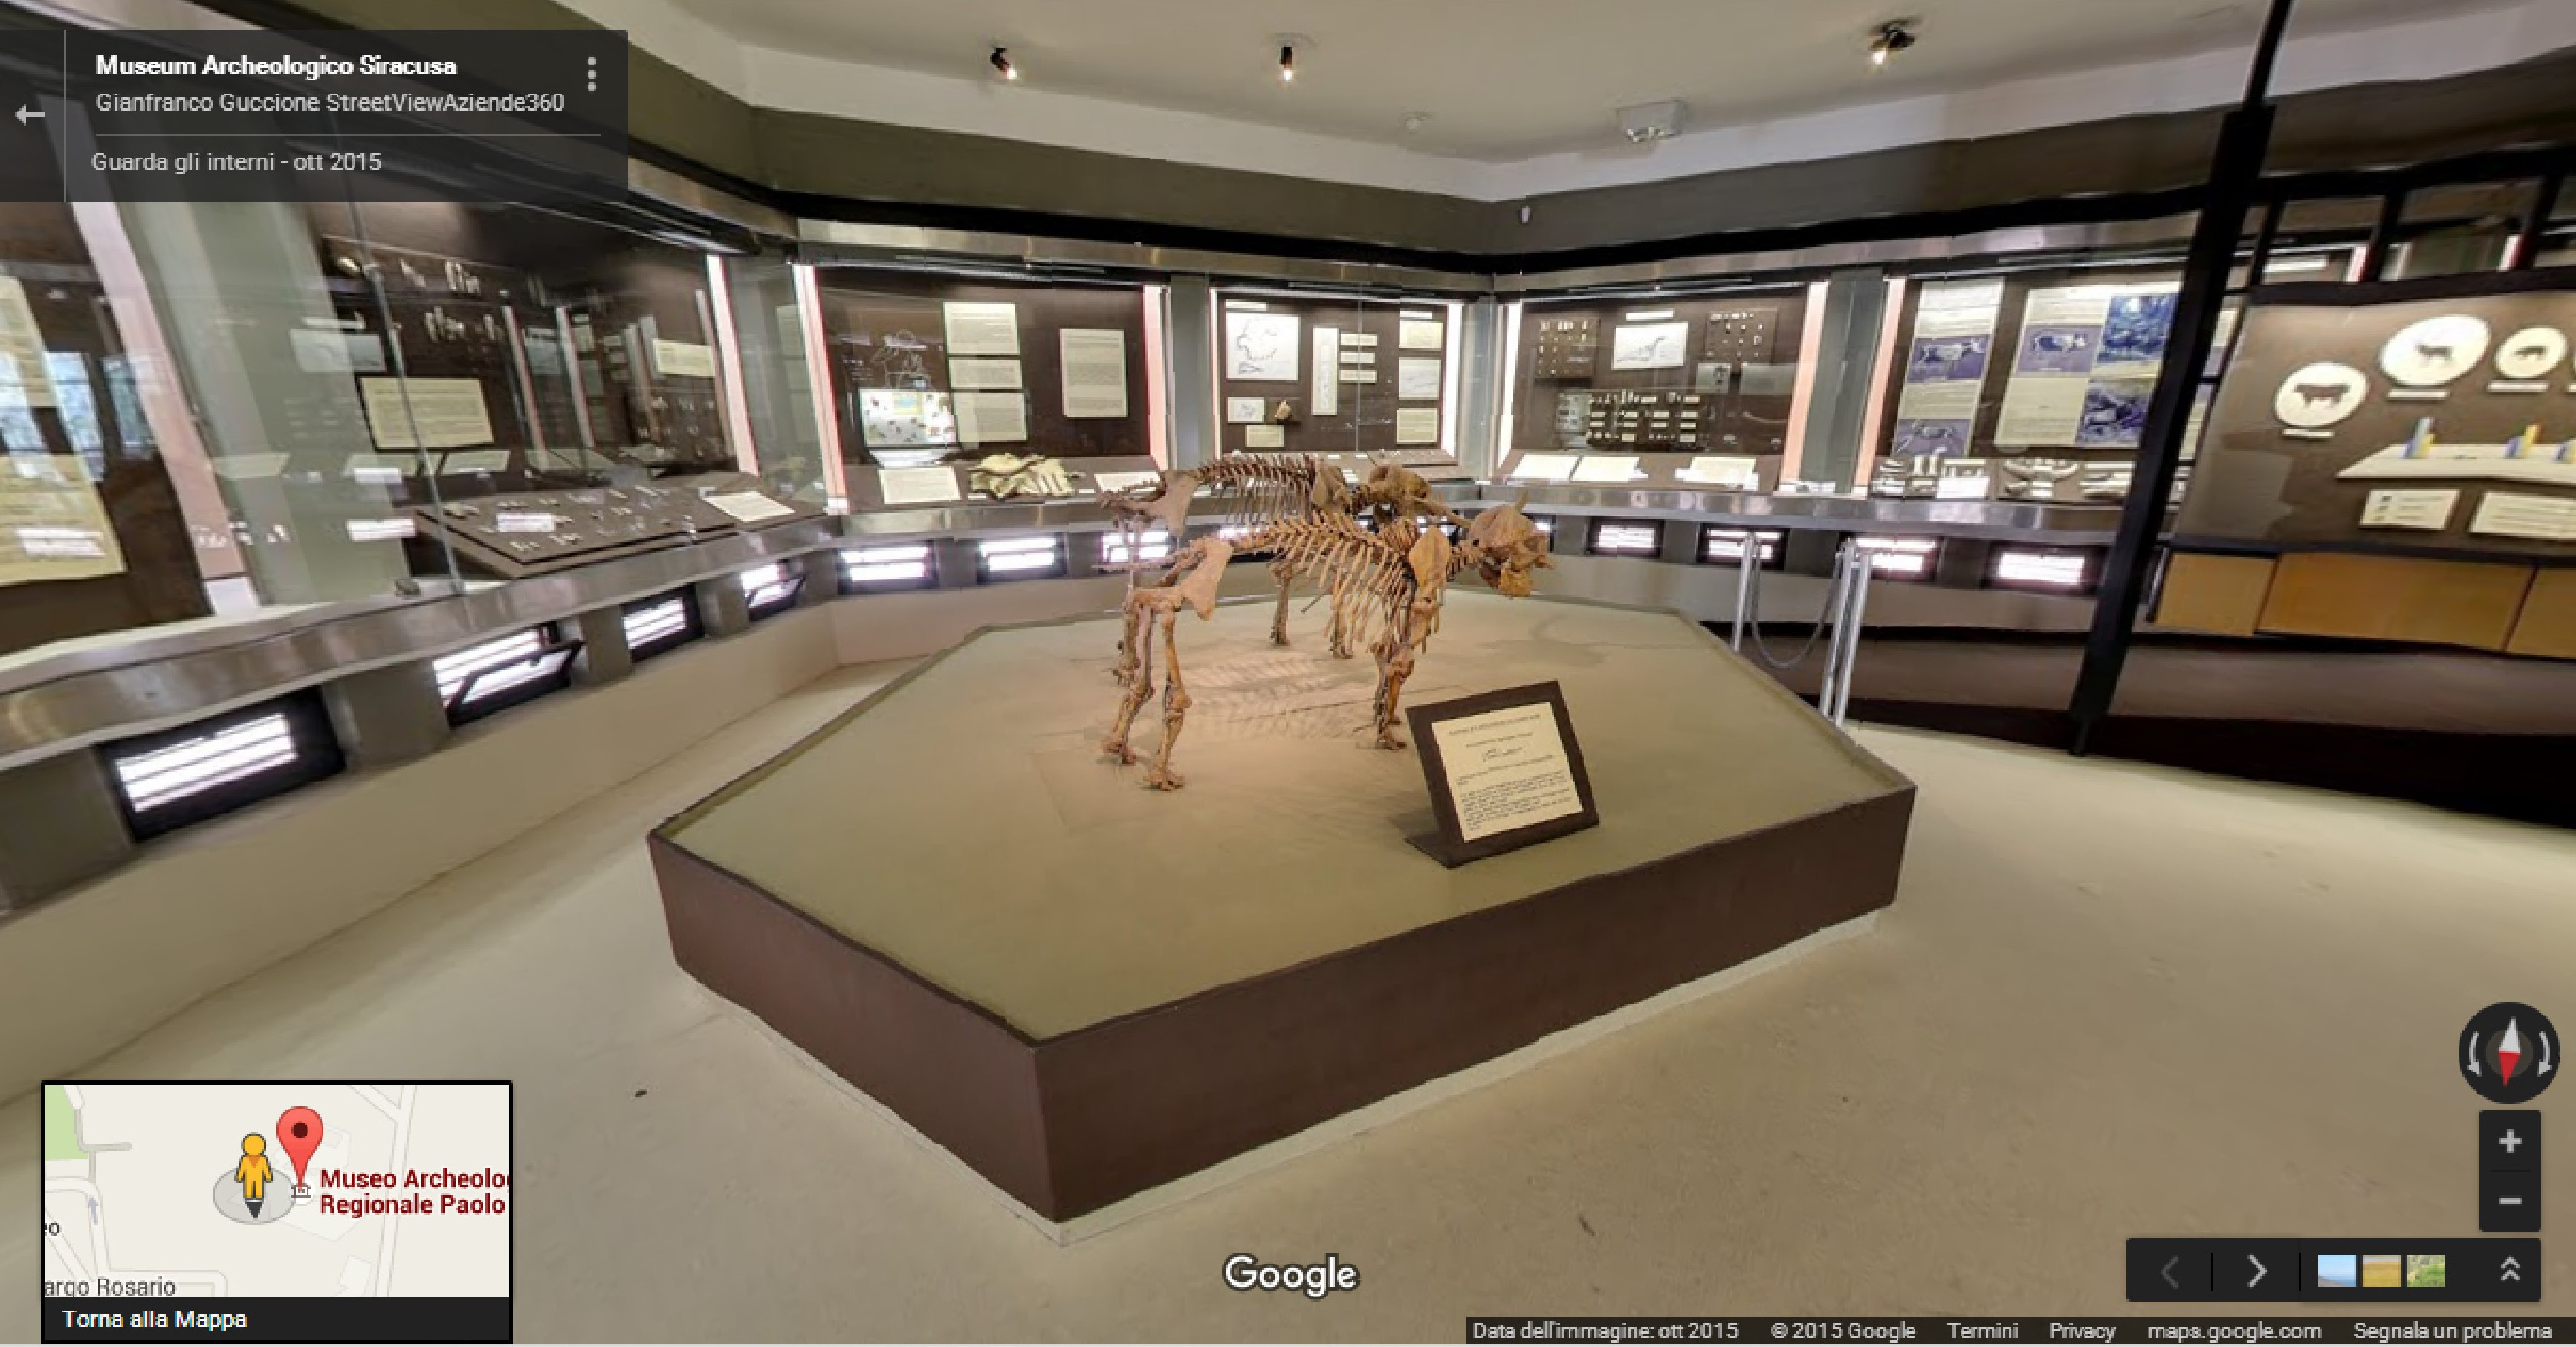
\includegraphics[width=\columnwidth]{EAGLE2016BONACINIPilotprojectatPaoloOrsiMuseum-img002.jpg}
\caption{360° tour of Sector A: a couple of casts of dwarf elephants from Spinagallo cave. }
\label{fig:2}
\end{figure}


In the Sector B1 remote users can admire findings from the first colonies founded by the Greeks in eastern Sicily
(Naxos, Zancle, Leontinoi, Katane, Megara Hyblaea) with some of the most important Greek masterpieces, as the naked
sculptures of young men from Leontinoi and Megara Hyblaea.

The B2 Sector introduces the visitor to the archaeological finds from the city of Syracuse, from its foundation to
classical age. Here the most important spaces are those dedicated to the architecture of archaic and classical temples
(Athenaion, Ionic temple, Olympeion and Apollonion), to the statuary and the terracotta findings from urban excavations
during the last decades (Piazza Duomo, Ortigia, Piazza della Vittoria) and to the urban and ex-traurban necropolis
(Fusco, Giardino Spagna) with rich funerary kits. \ 

\begin{figure}[!bp]
\centering
 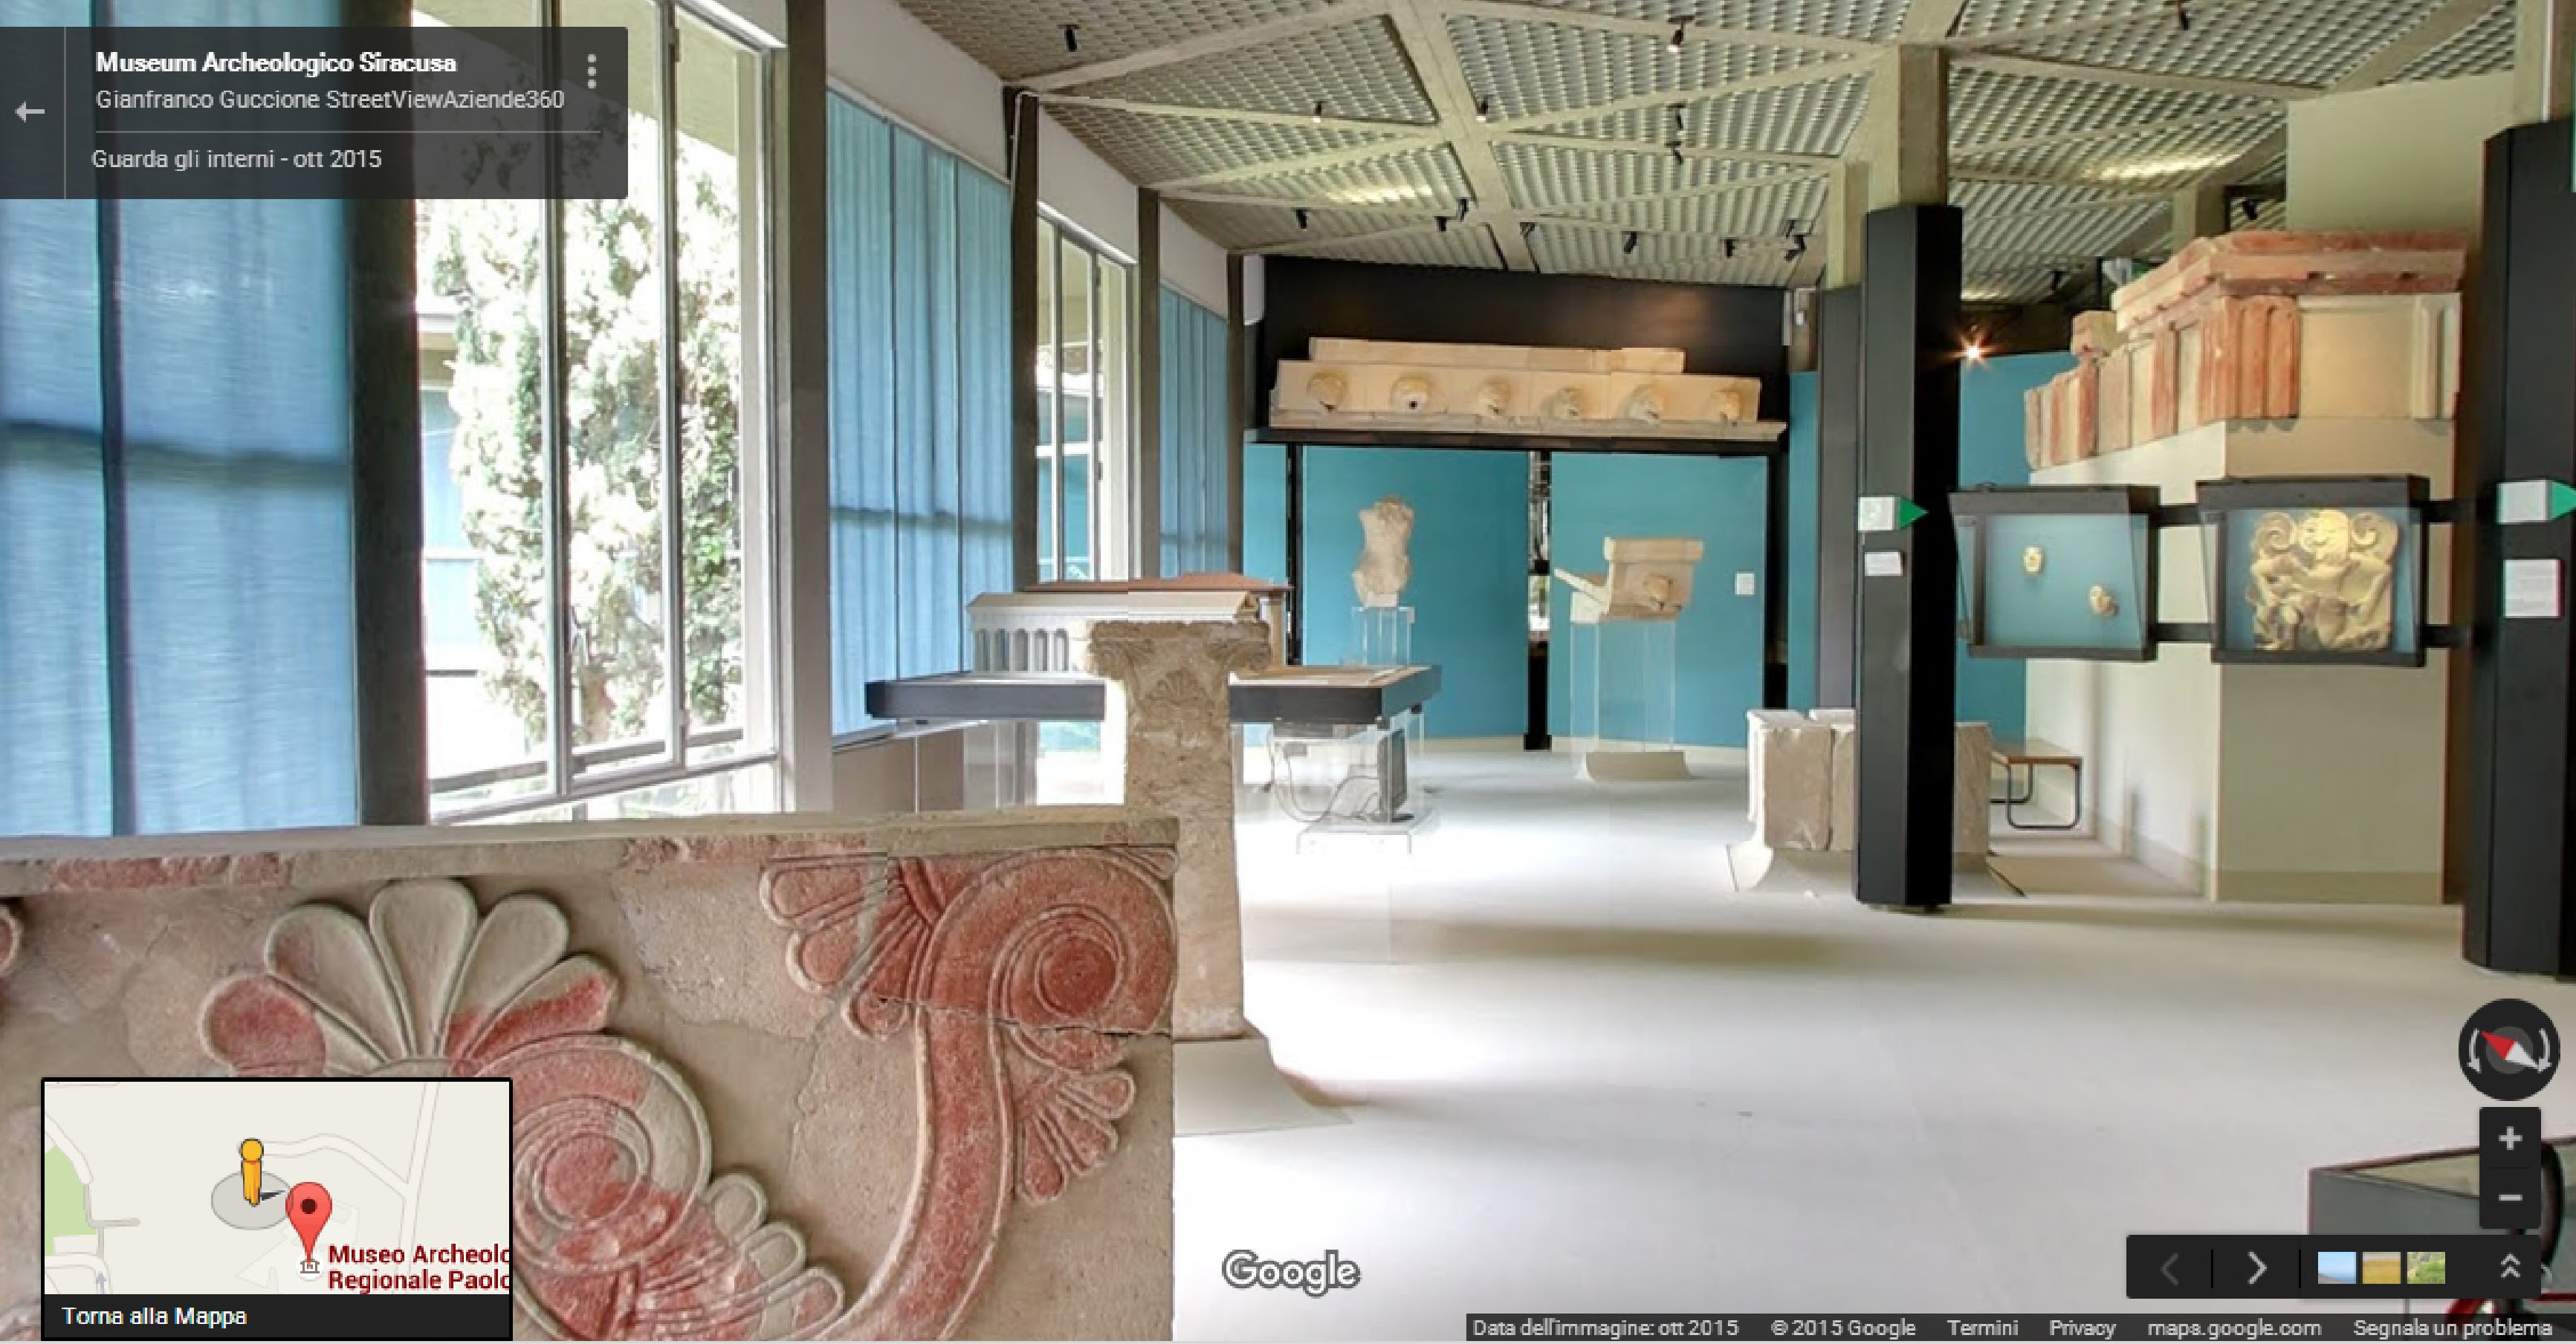
\includegraphics[width=\columnwidth]{EAGLE2016BONACINIPilotprojectatPaoloOrsiMuseum-img003.jpg}
\caption{360° tour of Sector B2: the findings from Athenaion and Ionic temple in Syracuse.}
\label{fig:3}
\end{figure}

Sector C is dedicated to the colonies founded by Syracuse - Eloro (670 B.C.), Akrai (664 B.C.), Kasmenai (644 B.C.) and
Camarina (598 B.C.) -, to Gela (689 B.C.) and Agrigento (580 B.C.), the largest colonies of south-eastern Sicily with
their ceramics, architectural remains of temples, findings from sanctuaries and necropolis, as well as finds from other
indigenous hellenized centres. 

Sector D on the second level contains finds from the Hellenistic age to the Roman period, including statuary, beautiful
portraits from the Roman age, architectural pieces, ceramics, mosaics, cinerary urns and various handcrafts. 

\begin{figure}[!bp]
\centering
 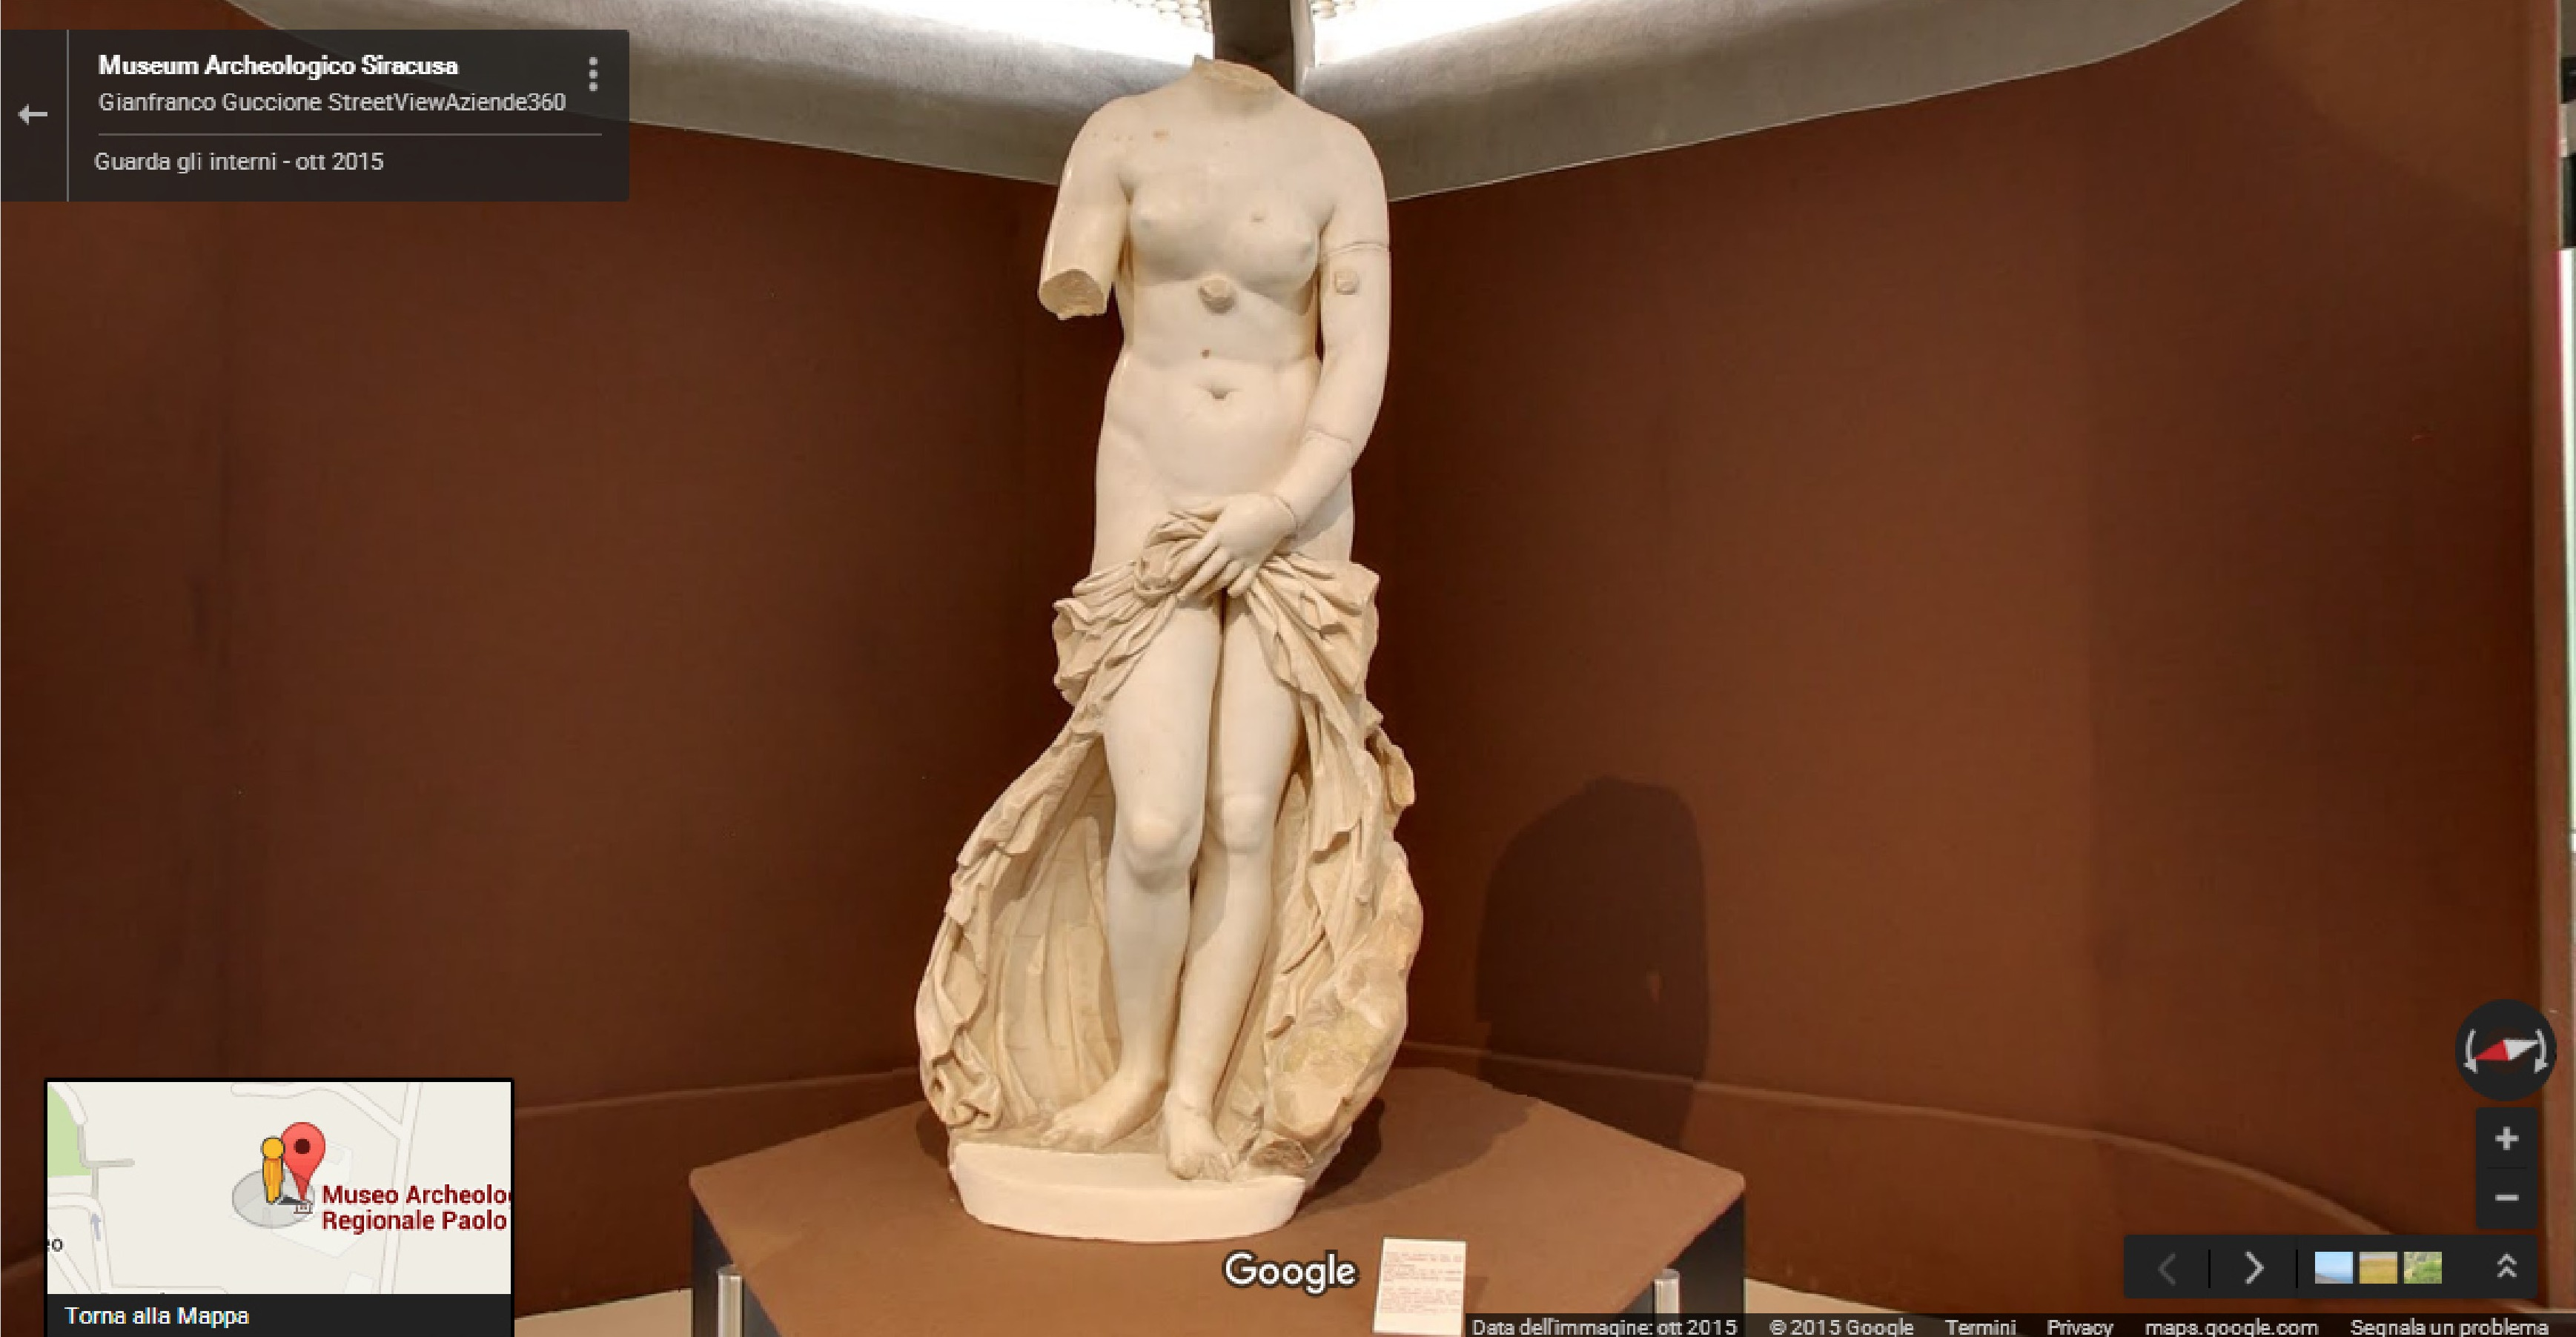
\includegraphics[width=\columnwidth]{EAGLE2016BONACINIPilotprojectatPaoloOrsiMuseum-img004.jpg}
\caption{360° tour of Sector D: the Venus Landolina.}
\label{fig:}
\end{figure}


They document the multiple aspects of life in Syracuse and come from urban necropolis from III-II century B.C. Here are
masterpieces like the wonderful statue of the Venus Anadiomene, called Venus Landolina, here in Fig.~\ref{fig:4}.

In Sector F finds from the various catacombs in the city are on show, documenting life in the Christian era. Here is the
Sarcophagus of Adelphia, a Christian marble sarcophagus found in the Rotunda of Adelphia inside the Catacombs of San
Giovanni, just near the museum.




\subsubsection{360° virtual tours of archaeological selected objects}


The Museum staff has selected 12 objects along the path between the two levels, which can be linked as points of
interest placed on the Museum map - where the remote user can identify sectors, plans and POI - with virtual 360° tours
equipped with labels with captions and descriptive texts.

Here are the selected objects:

\begin{description}
\item[From Sector A:] 

\begin{description}
\item[1] A foot-cup dated to the 15th century B.C., relevant to the facies of Rodì-Tindari and coming from Vallelunga, in the province of Caltanissetta. 
\end{description}


\item[From Sector B1:] 

\begin{description}
\item[2] A red-figured wedding lebes, attributed to Painter of Siracusa 47099, dated to 360-340 B.C. from Lentinoi. 
\end{description}


\item[From Sector B2:] 

\begin{description}
\item[3] A proto-corinthyan oinochoe, dated to 670 B.C., coming from the excavations in Piazza Duomo; 
\item[4] A plastic Corinthian vase in the form of a lion, dated 610-590 B.C., from the Garden Spain Necropolis; 
\item[5] An Attic black-figured calix-crater, by the Antimene Painter in 520 B.C., coming from the Garden Spain Necropolis; 
\item[6] An Attic black-figured Panathenaic amphora, dated to the middle of the 6th century B.C., coming from excavations in Viale Paolo Orsi; 
\item[7] A terracotta bidder statuette, dated to the 4th century B.C., coming from the sacred votive deposit in Piazza della Vittoria. 
\end{description}

\item[From Sector C:]

\begin{description}
\item[8] A red-figured bell-shaped krater, coming from Camarina, produced in the workshop of the Athenian painter Polignoto, around 440-430 B.C., decorated on the principal side with the Delphic triad (Apollo, Artemis and Latona); 
\item[9] An Attic red-figured lekythos, coming from the necropolis of Capo Soprano near Gela, dated to 470 B.C. and realized according to the manner of the London painter E342; 
\item[10] The Ephebus of Adrano, a small bronze athlete, dated to the first half of the 5th century B.C., generally thought to be a scaled-down copy of a large bronze original by the famous Greek sculptor Pythagoras. 
\end{description}


\item[From Sectors D:]

\begin{description}
\item[11] A small Hellenistic terracotta boat in the shape of a pistrix (sea monster), from the Fusco necropolis in Syracuse. 

\end{description}

\item[From Sector F:]

\begin{description}
\item[12] The Nassiane inscription Fig.~\ref{fig:4}, a curious marble disk, from the Catacombs of San Giovanni.
\end{description}


\end{description}

Fixed on tripods the reflex camera with a quadrangolar lens, the objects have been photographed flipping them on a
graduated portable rolling disk. Each 360° object virtual tour took a number of about 88 shots, for a total of 1.062
shots, mounted with specific software. In this way the remote user, clicking on the preview pictures, can admire the
selected object in all its sides, by moving the mouse on the right and left and zoom in-out.




\subsubsection{360° virtual tours of Nassiane inscription}


The last selected object we present here is a disk from Sector F: it is a marble disk, discovered by Paolo Orsi in the
Catacombs of San Giovanni in 1894 \citep[509-510]{Orsi1895}, decorated by a wreath of laurel leaves on one side; the other
side was reused in the 4th century A.D. for the funerary inscription of Nassiane, woman who died at age 32 in God
faith. 

This object, which the remote user can observe with a 360° virtual tour, has been selected both for the peculiar reuse
and because it documents the religious syncretism of the early centuries of Christianity. Re-using of architectural is
well documented in the catacombs of Syracuse \citep{Sgarlata2013}. It was found shattered in front of a burial, distinct
from others, known as ``the Saint's Tomb'' \citep[40-44]{Sgarlata2004}. 



\begin{figure}[!bp]
\centering
 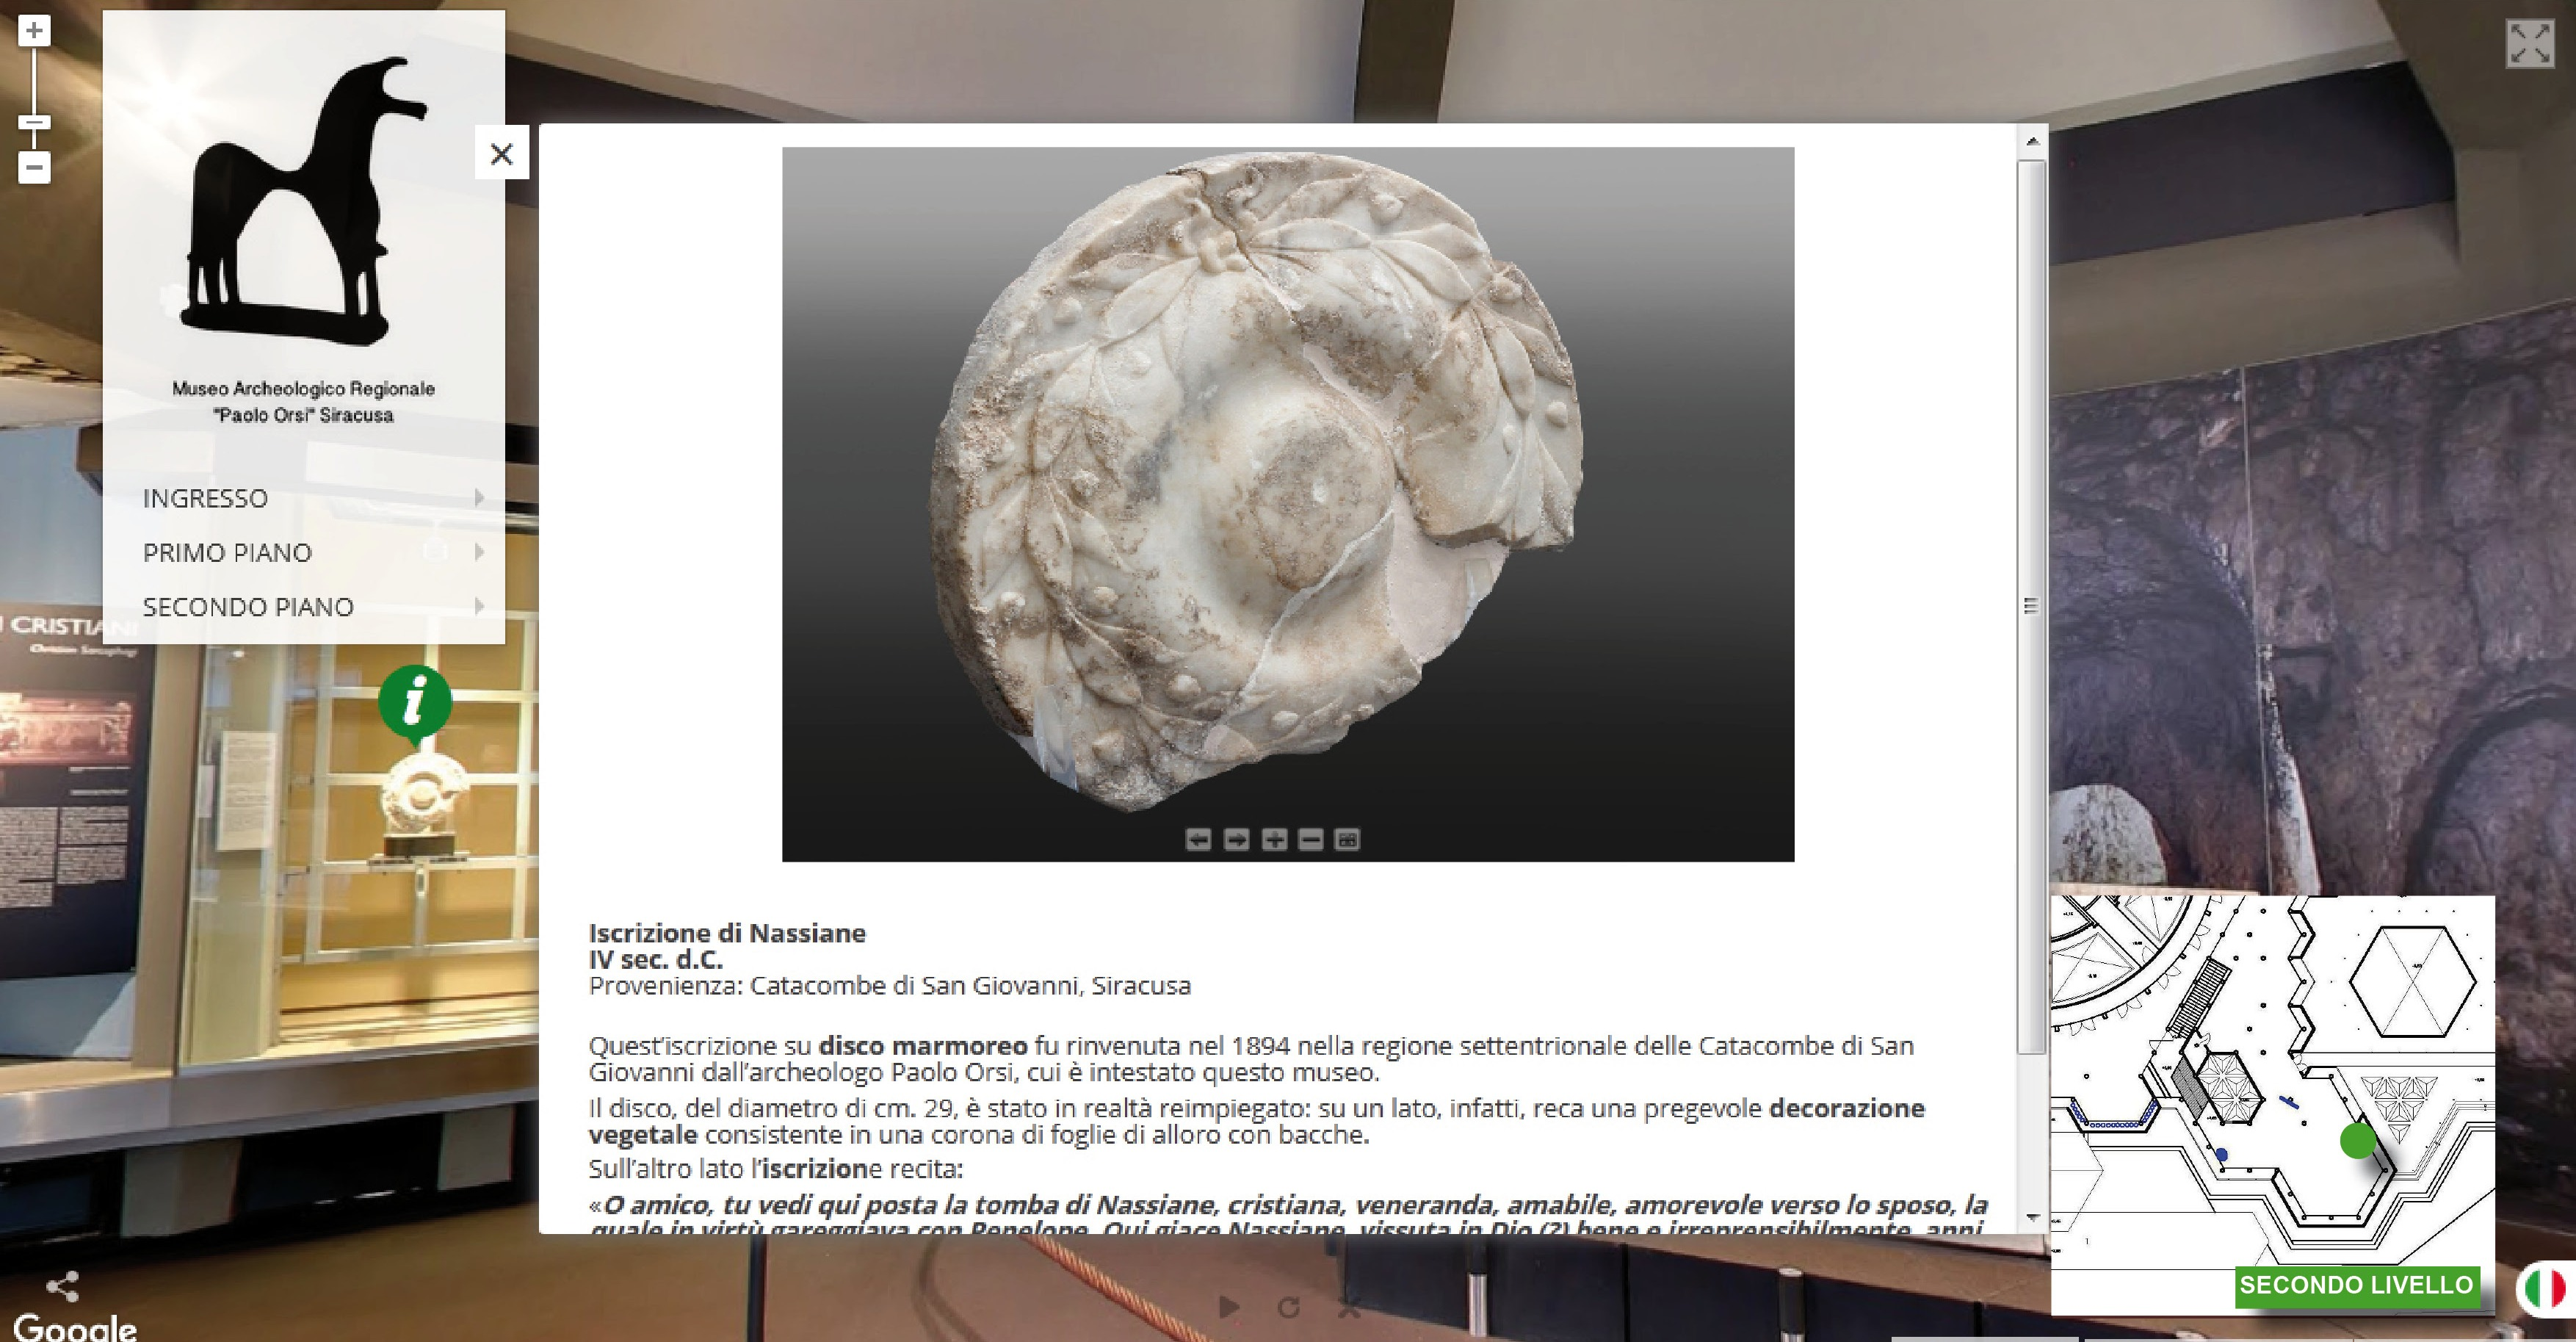
\includegraphics[width=\columnwidth]{EAGLE2016BONACINIPilotprojectatPaoloOrsiMuseum-img005.jpg}
\caption{360° tour of the Nassiane inscription.}
\label{fig:5}
\end{figure}


This is the Greek text: 

\begin{quotation}


\begin{otherlanguage*}{greek}
chrismon ς χριστ<ι>ανῆς σεμνῆς ἀγανóφρονος [ἠδ]ὲ φιλάνδρου Nασσιανῆς τύμβον εἰσορᾷς, φίλε, κίμενον [ὣδε ἥ]τις σεμνοσύνῃσιν [ἐριζε]το Πηνελοπίῃ palma chrismon ἐνθάδε κῖτε [Nασσ]ιανή, ζήσασα [ἐν Θ(ε)ῷ] καλῶς καὶ ἀμέμπτως ἒτη λβ´, μῆνας ι´.
\end{otherlanguage*}

\end{quotation}



The inscription says: ``Oh friend, you see here the tomb of Nassiane, Christian, ripe, sweet, fond of her husband, who
competed for virtue with Penelope. Here lies Nassiane, she lived well and blamelessly in God (?), 32 years and 10
months''. This inscription documents such as epigraphic formulas affected by religious syncretism (syncretism generally
means that a complex of phenomena and concepts derive from the meeting and fusion of different religious forms) between
Pagans and Christians, for which a Christian like Nassiane could have competed in life with Penelope, the hero
Odysseus’ wife and symbol of marital devotion. Its circular shape suggested that it was a table for the ritual of
refrigerium, the funeral feast that symbolically was consumed with the dead, even this syncretic practice \ dates back
to the pagan world \citep{Sgarlata2013}, \citep{Scandurra2014}.


\begin{figure}[!bp]
\centering
 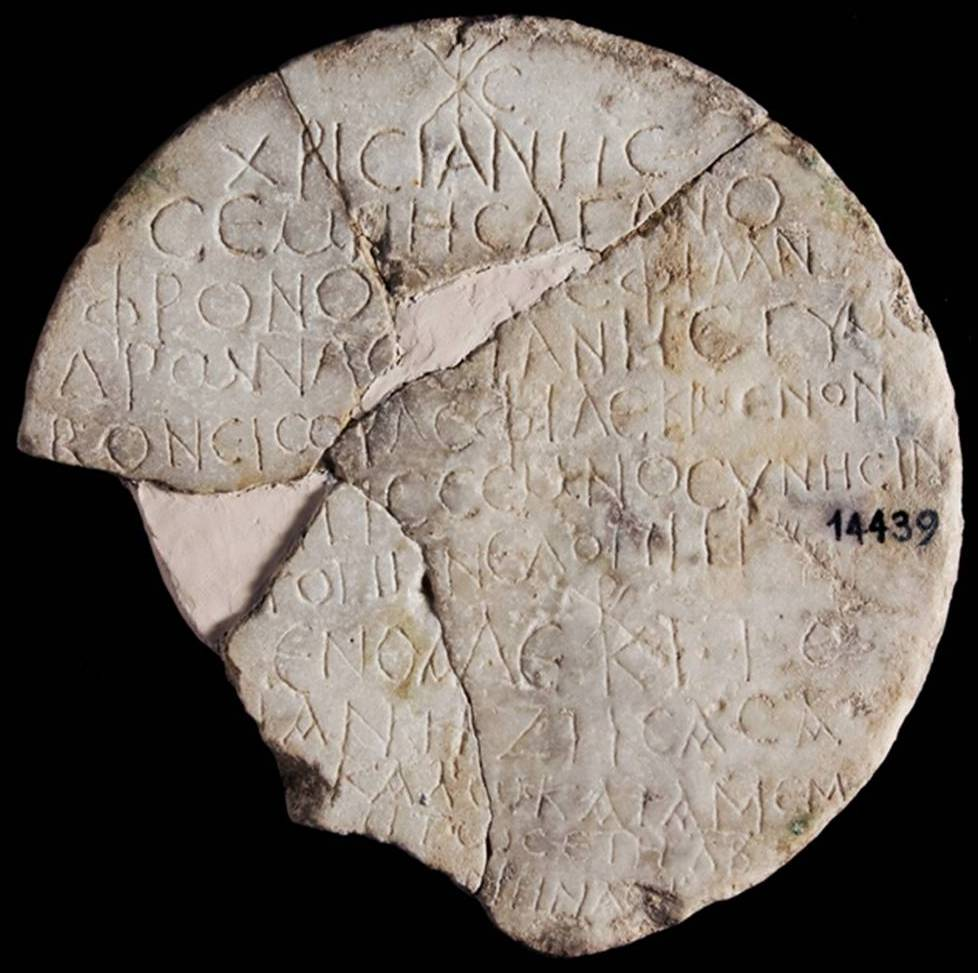
\includegraphics[width=\columnwidth]{EAGLE2016BONACINIPilotprojectatPaoloOrsiMuseum-img006.jpg}
\caption{ The Nassiane inscription, recto (courtesy by the ``Paolo Orsi'' Museum). }
\label{fig:6}
\end{figure}

\section{Conclusions}


As discussed elsewhere (Bonacini 2013 and 2014), Google is undoubtedly the most active entity in the world committed to
preservation, dissemination and promotion of cultural heritage, well above any public institution, through an
unparalleled campaign of digitization open to users’ collaboration. This could happen because Google itself has an
incomparable capacity of economic investment. Even large international projects of digitization (such as Europeana
itself) \ are not able to compete with Google.

Therefore, after initial hesitation towards these Google’s initiatives, now most of museums and cultural institutes in
the world have seen in Google a partner that enables them to progress in the online visibility and in the process of
heritage digitization.

Regarding the project here presented, which concerns one of the two selected sites, we can rightfully say that it is the
first archaeological museum in the world - needless to say, the first museum in Sicily - entirely browsable on Google
Maps platforms with a virtual tour in all exhibition halls and 360° virtual tours with integration of captions and full
description of artworks.

In the near future we hope to allow 360° visualization of a greater number of objects, with their accompanying captions
translated at least in English and in audio version.

Thanks to this project we hope that Google itself could realize how the time has come to ``rejuvenate'' the Google Maps
Street View system, allowing enabled users to apply additional content on the maps.

However, the wide interoperability between Google software the development of new solutions and the integration of
geo-referenced results in the page results on the search engine continues unabated: the ``Paolo Orsi'' Museum - and with
the museum, the city of Syracuse and the whole of Sicily – will surely take advantage of this new tool for its
visibility.






\section*{Acknowledgement}


To Mr. Gianfranco Guccione (\url{http://www.airworks.it/}) goes my heartfelt and deep thanks for having proposed to me this
project and having concluded it together, with the only aim of enhancing the Cultural Heritage in Sicily.

I would like to thank some people, because without them it would not have been easy to achieve this result: Professor
Mariarita Sgarlata, formerly Regional Minister of Cultural Heritage and Sicilian Identity; Dr. Sergio Gelardi, formerly
General Director of Cultural Heritage, Dr. Gaetano Pennino, current General Director of Cultural Heritage; Dr. Enrico
Carapezza, Area Manager for General Affairs of the Department of Cultural Heritage and Dr. Maria Pia Bottino, formerly
member of the cabinet of Regional Minister of Cultural Heritage and Sicilian Identity.

I warmly thank all staff of the ``Paolo Orsi'' Regional Archaeological Museum in Syracuse for the great availability and
friendship shown to me and Mr. Guccione: Dr. Gioconda Lamagna, executive head of the Museum, Dr. Angela Maria Manenti,
head of relations with the public, all the archaeologists Dr. Anita Crispino, Dr. Agostina Musumeci and especially Dr.
Giuseppina Monterosso, tireless in supporting the project at any time and formerly member of the cabinet of Regional
Minister of Cultural Heritage and Sicilian Identity.

Many thanks to Dr. Peter Shishkov, Google Business Photos/Street View Indoor European Coordinator, for supporting Mr.
Guccione’s initiative.

To the University of Catania, to the Chancellor Prof. Giacomo Pignataro and to the Humanities Department Director Prof.
Giancarlo Magnano San Lio deserve my thanks for allowing me to work on this project.

My deepest gratitude goes to my friend Prof. Annalisa Bonica for the patience she has showed in correcting this
article.

This publication has been made on concession of the Regional Minister of Cultural Heritage and Sicilian Identity;
archaeological findings and plans presented here are exclusive property of the ``Paolo Orsi'' Regional Archaeological
Museum in Syracuse and it not allowed to be copied or duplicated by any means.

\nocite{Farman}
\bibliographystyle{sapauth-eng}
\bibliography{../../EAGLE}

\end{document}
